%
\section{Transform Once: The \ourmethod{} Recipe}\label{sec:t1rec}

With \ourmethod{}, we introduce major modifications to the way FDMs are designed and optimized. In particular, \ourmethod{} is defined, inferred and trained directly in the frequency domain with only a \textbf{single} direct transform required to process data. Hence follows the name: \textit{transform once} (\ourmethod{}).


\paragraph{Direct learning in the frequency domain} 


Consider two signals $x\in\cD_n$, $y\in\cD_n$ and suppose there exists a function $\varphi:\cD_n\rightarrow\cD_n$ mapping $x$ to $y$, i.e.
%
\[
    \quad y = \varphi(x).
\]
%
Then, there must also exist another function $\psi:\cD_k\rightarrow\cD_k$ that relates the spectra of the two signals, i.e. $Y = \psi(X)$
%
being $X = \cT(x)$ and $Y = \cT(y)$. In particular,
%
\[
    \varphi(x) = \cT^{-1} \circ \psi \circ \cT(x)~~\Leftrightarrow~~\cT\circ\varphi(x) = \psi \circ \cT(x)
\]
%
It follows that, from a learning perspective, we can aim to approximate $\psi$ directly in the $k$-space rather than $\varphi$ in the $n$-space. To do so, we define a learnable parametric function $f_\theta:\cD_k\rightarrow\cD_k$ and train it to minimize the approximation error $J_\theta$ of the output signal spectrum $Y$ in the $k$-space. Given a distribution $p(x)$ of input signals, \ourmethod{} is characterized by the  following nonlinear program
%
\begin{equation}\label{eq:2}
    \tikzstyle{block} = [draw, fill=blue!20!white, rectangle, rounded corners]
    \tikzstyle{sum} = [draw, fill=blue!20, circle, node distance=1cm]
    \tikzstyle{container} = [draw, rectangle, inner sep=0.15cm, fill=gray!20,minimum height=1cm, dotted, rounded corners, thick]
    \begin{tikzpicture}[>=latex', baseline=(current  bounding  box.center)]
        % nodes
        \node at (-3.5,-0.5) {$
        	\begin{aligned}
        \min_{\theta}~~& \bE_{x,y}\left[\| \cT(y)- \hat Y \|\right]\\
        \st~~& \hat Y = f_{\theta} \circ \cT(x)\\
        ~~& x \sim p(x) \\
        ~~& y = \varphi(x) 
    \end{aligned}
        $};
        \node (x) at (0, 0) {$x$};
        \node (y) at (0, -1) {$y$};
        \node (X) at (1.75, 0) {$X$};
        \node (Y) at (1.75, -1) {$Y$};
        \node (Y_) at (3.35, .3) {$\hat Y$};
        %\node (loss) at (5.5,0) {Loss};
        \node [block, blur shadow={shadow blur steps=5}] (T) at (.8, 0) {$\mathcal{T}$};
        \node [block, blur shadow={shadow blur steps=5}] (T_) at (.8, -1) {$\mathcal{T}$};
        \node [block, blur shadow={shadow blur steps=5}, fill=green!20] (f) at (2.75, 0) {$f_\theta$};
        \node [block, blur shadow={shadow blur steps=5}, fill=yellow!80!black] (J) at (4, 0) {$J_\theta$};
        %
        %
        \begin{scope}[on background layer]
        \node [container,fit=(x) (y) (T) (T_)] (preproc) {};
        \node [container,fit=(X) (Y), fill=blue!20!gray!20] (data) {};
        \end{scope}
        % lines
        \draw [->] (x) -- (T);
        \draw [->] (y) -- (T_);
        %\draw [->] (T) -- (f);
        \draw [-] (T) -- (X);
        \draw [->] (X) -- (f);
        \draw [->] (f) -- (J);
        %\draw [->] (J) -- (loss);
        %\draw [->] (T_) -| (J);
        \draw [-] (T_) -- (Y);
        \draw [->] (Y) -| (J);
        %
        %\node[] at (.85, .85) {offline pre-processing};
    \end{tikzpicture}
\end{equation}
%
If $\cT$ is a DFT, the above turns out to be a close approximation (or equivalent, depending on the function class of $f_\theta$) to the minimization of $\|y - \hat{y}\|$ in $n$-space by the \textit{Parseval-Plancherel identity}.


\begin{restatable}[Parseval-Plancherel Identity {\cite[pp. 223]{stein2011fourier}} ]{thm}{parseval} \label{prop:parseval}
    Let $\cT$ be the normalized DFT. Given a signal $v\in\cD_n$ and its transform $V = \cT(v)$, it holds $\|v\| = \|V\|$.
\end{restatable}
%
This result also applies to any other norm-preserving transform $\cT$, e.g.  a normalized type-\textsc{II} DCT \citep[pp. 679]{oppenheim1999discrete}. For the linear transforms considered in this work, $\cT(x) = Wx,~W\in\bC^{N\x N}$, condition for Th. \ref{prop:parseval} to hold is $W$ to be orthonormal, i.e. $W^*W = \Id$.
%


Note that \ourmethod{} retains, in principle, the same universal approximation properties of FNOs \citep{kovachki2021universal} as $f_\theta$ is allowed to operate on the entirety of the input spectrum. Given enough capacity, $f_\theta$ can arbitrarily approximate $\psi$, implicitly reconstructing $\varphi$ via $\cT^{-1}\circ f_\theta\circ\cT$.

%
\paragraph{Speedup measurements}
%
We provide a concrete example of the effect of pruning redundant transforms on computational costs. We measure wall-clock inference time speedups of depth $d$ \ourmethod{}
\[
\text{\ourmethod{}}(x):= f_{d} \circ \cdots\circ f_2 \circ f_1 \circ \cT(x)
\]
over an equivalent depth $d$ FNO with layers \eqref{eq:1}. The only difference concerns the application of transforms between layers. 

 \cref{fig:speedup-contour-2d} provides the speedups on two-dimensional signals: on the left, we fix model depth $d=6$ and investigate the scaling in signal width (i.e. number of channels) and signal resolution. On the right, we fix signal width to be $32$ and visualize the interaction of model depth and signal resolution. For common experimental settings e.g. resolutions of $64$ or $128$, $6$ layers and width $32$, \ourmethod{} is at least $10$ x faster than other FDMs. It will later be shown (\cref{sec:experiments}) that \ourmethod{} also preserves or improves on predictive accuracy of other FDMs across tasks.

\begin{wrapfigure}[17]{r}{0.45\textwidth}\label{clean_speedups}
    \centering
    \vspace{-3mm}
    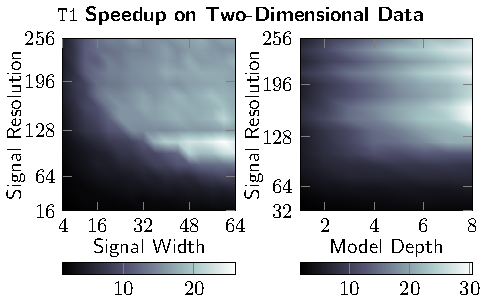
\includegraphics[width=0.9\linewidth]{drawings/speedup_2d.pdf}
    \vspace{-5mm}
    \caption{\footnotesize Speedup in a forward pass of \ourmethod{} over FNOs sharing the same transform $\cT$ (DFT) on two-dimensional signals of increasing resolution. The speedup for a given configuration (point on the plane) is shown as background color gradient. The improvement grows with signal width, resolution and model depth. }
    \label{fig:speedup-contour-2d}
\end{wrapfigure}

When \ourmethod{} is not preceded by online preprocessing steps for inputs $x$, such as other neural networks or randomized data augmentations, the transform on $\cT(x)$ can be done once  on the dataset, amortizing the cost over training epochs, and increasing the speed of \ourmethod{} further.




\paragraph{Choosing the right transform}\label{par:choosing}

The transform $\cT$ in \ourmethod{} is chosen to be in the class of \textit{Discrete Cosine Transforms} (DCTs) \citep{ahmed1974discrete,strang1999discrete}, in particular the normalized DCT-II, which can also be computed $\mathcal{O}(N \log N)$ via FFTs \citep{makhoul1980fast}. DCTs provide effective representations of smooth continuous signals \citep{trefethen2019approximation} and are the backbone of modern lossy compression methods for digital images.

Although other transforms are available, we empirically observe DCT-based {\tt T1} to perform best in our experiments. This phenomenon can be explained by the sparsity and energy distribution properties of the transformed spaces, an intrinsic property of the specific dataset and chosen transform. This is in line with results of classic signal processing and compression literature. Particularly, DCT features are known to have a higher energy compaction than their DFT counterparts in a variety of domains, from natural images \citep{yaroslavsky2014fast} to audio signals \citep{soon1998noisy}. Energy compaction is often the decisive factor in choosing a transform for downstream tasks.  

Letting $\mathcal{T}$ be a real-valued transform in {\tt T1} architectures preserves compatibility between $f_{\theta}$ and existing architectures e.g., models pre-trained on natural image datasets. 


\subsection{Reduced-Order \ourmethod{} Model and Irreducible Loss Bound}\label{subsec:inverse}

We seek to leverage structure induced in $\cD_k$ by $\cT$. To this end we allow \ourmethod{}, similarly to \eqref{eq:1}, to modify specific elements of $X$ and consequently trasform only certain frequency components of $x$ (and $y$). 
%

The reduced-order \ourmethod{} model is designed to operate only on $m<N$ elements (selected by $S_m\in\R^{N\times m}$) of the input $k$-space, i.e. on a \textit{reduced} $k$-space $\cD_m\equiv\R^m$ of lower dimension.
Thus, we can employ a smaller neural network $\gamma_\theta:\cD_m\rightarrow\cD_m$ for mapping $S_m X$ to the corresponding $m$ elements $S_m Y$ of the output $k$-space. Thus, training involves a truncated objective that compares predictions with elements in the output signal spectrum also selected by $S_m$:
%
\begin{equation}\label{eq:3}
    \tikzstyle{block} = [draw, fill=blue!20!white, rectangle, rounded corners,  blur shadow={shadow blur steps=3}, thick]
    \tikzstyle{el} = [draw, fill=gray!20, circle, blur shadow={shadow blur steps=3}, minimum size=.25cm, inner sep=0pt, outer sep=0pt, thick]
    \tikzstyle{container} = [semithick, draw, rectangle, inner sep=0.1cm, rounded corners, fill=blue!10!gray!10]
    \begin{tikzpicture}[>=latex', baseline=(current  bounding  box.center)]
        % \node[el] at (0,0) (x0) {};
        % \node[el] at (-.5,0) (x1) {};
        % \node[el] at (-1,0) (x2) {};
        % \node[el] at (-1.5,0) (x3) {};
        % \node[el] at (-2,0) (x4) {};
        % \node[el] at (-2.5,0) (x5) {};
        % \node[el] at (-3,0) (x6) {};
        % %
        % \node[el] at (0,-.75) (X0) {};
        % \node[el, fill=blue!50] at (-.5,-.75) (X1) {};
        % \node[el, fill=blue!50] at (-1,-.75) (X2) {};
        % \node[el] at (-1.5,-.75) (X3) {};
        % \node[el] at (-2,-.75) (X4) {};
        % \node[el, fill=blue!50] at (-2.5,-.75) (X5) {};
        % \node[el] at (-3,-.75) (X6) {};
        % %
        % \node[el, fill=blue!50] at (0,-1.5) (X0s) {};
        % \node[el, fill=blue!50] at (-.5,-1.5) (X1s) {};
        % \node[el, fill=blue!50] at (-1,-1.5) (X2s) {};
        % %
        % \node[block] at (-.5, -2.25) (gamma) {$\gamma_\theta$};
        % %
        % \node[el, fill=red!50] at (0,-3) (Yh0) {};
        % \node[el, fill=red!50] at (-.5,-3) (Yh1) {};
        % \node[el, fill=red!50] at (-1,-3) (Yh2) {};
        % %
        % \node[] at (.5, 0) {$x$};
        % \node[] at (.5, -.75) {$X$};
        % \node[] at (.75, -1.5) {$S_mX$};
        % \node[] at (.5, -3) {$\hat Y$};
        % %
        % \begin{scope}[on background layer]
        %     \node [container,fit=(X0s) (X1s) (X2s)] {};
        %     \node [container,fit=(Yh0) (Yh1) (Yh2)] {};
        %     \node [container,fit=(X0) (X1) (X2) (X3) (X4) (X5) (X6)] {};
        %     \node [container,fit=(x0) (x1) (x2) (x3) (x4) (x5) (x6)] {};
        % \end{scope}
        % %
        % \path[-] (x0) edge (X0)
        %          (x1) edge (X1)
        %          (x2) edge (X2)
        %          (x3) edge (X3)
        %          (x4) edge (X4)
        %          (x5) edge (X5)
        %          (x6) edge (X6);
        % \path[-] (X1) edge (X0s)
        %          (X2) edge (X1s)
        %          (X5) edge (X2s);
        % \path[-] (X0s) edge (gamma.north)
        %          (X1s) edge (gamma.north)
        %          (X2s) edge (gamma.north);
        % \path[-] (gamma.south) edge (Yh0)
        %          (gamma.south) edge (Yh1)
        %          (gamma.south) edge (Yh2);
        %
        \node[el] at (0,0) (x0) {};
        \node[el] at (0,-.5) (x1) {};
        \node[el] at (0,-1) (x2) {};
        \node[el] at (0,-1.5) (x3) {};
        \node[el] at (0,-2) (x4) {};
        \node[el] at (0,-2.5) (x5) {};
        \node[el] at (0,-3) (x6) {};
        %
        \node[el] at (.75, 0) (X0) {};
        \node[el, fill=blue!50] at (.75,-.5) (X1) {};
        \node[el, fill=blue!50] at (.75,-1) (X2) {};
        \node[el] at (.75,-1.5) (X3) {};
        \node[el] at (.75,-2) (X4) {};
        \node[el, fill=blue!50] at (.75,-2.5) (X5) {};
        \node[el] at (.75,-3) (X6) {};
        %
        \node[el, fill=blue!50] at (1.5,0) (X0s) {};
        \node[el, fill=blue!50] at (1.5,-.5) (X1s) {};
        \node[el, fill=blue!50] at (1.5,-1) (X2s) {};
        %
        \node[block] at (2.25,-.5) (gamma) {$\gamma_\theta$};
        %
        \node[el, fill=red!50] at (3,0) (Yh0) {};
        \node[el, fill=red!50] at (3,-.5) (Yh1) {};
        \node[el, fill=red!50] at (3,-1) (Yh2) {};
        %
        \node[] at (0,.5) {$x$};
        \node[] at (.75,.5) {$X$};
        \node[] at (1.5,.5) {$S_mX$};
        \node[] at (3,.5) {$\hat Y$};
        %
        \path[-] (x0) edge (X0)
                 (x1) edge (X1)
                 (x2) edge (X2)
                 (x3) edge (X3)
                 (x4) edge (X4)
                 (x5) edge (X5)
                 (x6) edge (X6);
        \path[-] %(X1) edge (X0s)
                 ([xshift=1mm] X1.east) edge ([xshift=-1mm] X1s.west);
                 %(X5) edge (X2s);
        \path[-] (X0s) edge (gamma.west)
                 (X1s) edge (gamma.west)
                 (X2s) edge (gamma.west);
        \path[-] (gamma.east) edge (Yh0)
                 (gamma.east) edge (Yh1)
                 (gamma.east) edge (Yh2);
        \def\x{5};
        \def\y{-3};
        \node[el] at (\x,\y) (y0) {};
        \node[el] at (\x-.5,\y) (y1) {};
        \node[el] at (\x-1,\y) (y2) {};
        \node[el] at (\x-1.5,\y) (y3) {};
        \node[el] at (\x-2,\y) (y4) {};
        \node[el] at (\x-2.5,\y) (y5) {};
        \node[el] at (\x-3,\y) (y6) {};
        %
        \node[el] at (\x + 0,\y+.75) (Y0) {};
        \node[el, fill=green!50] at (\x -.5,\y+.75) (Y1) {};
        \node[el, fill=green!50] at (\x -1,\y+.75) (Y2) {};
        \node[el] at (\x -1.5,\y+.75) (Y3) {};
        \node[el] at (\x -2,\y+.75) (Y4) {};
        \node[el, fill=green!50] at (\x -2.5,\y+.75) (Y5) {};
        \node[el] at (\x -3,\y+.75) (Y6) {};
        %
        \node[el, fill=green!50] at (\x ,\y+1.5) (Y0s) {};
        \node[el, fill=green!50] at (\x -.5,\y+1.5) (Y1s) {};
        \node[el, fill=green!50] at (\x -1,\y+1.5) (Y2s) {};
        \node[] at (\x+.5, \y) {$y$};
        \node[] at (\x+.5, \y+.75) {$Y$};
        \node[] at (\x+.75, \y+1.5) {$S_mY$};
        \path[-] (y0) edge (Y0)
                 (y1) edge (Y1)
                 (y2) edge (Y2)
                 (y3) edge (Y3)
                 (y4) edge (Y4)
                 (y5) edge (Y5)
                 (y6) edge (Y6);
        \path[-] ([yshift=1mm] Y1.north) edge ([yshift=-1mm] Y1s.south);
        
        \node[el, fill=yellow!70!black] (J) at (\x-.5,-.5) {};
        \node[] at (\x,-.5) {$J_\theta$};
        
        \path[->] ([yshift=1mm] Y1s.north) edge ( J.south);
        \path[->] ([xshift=1mm] Yh1.east) edge ( J.west);
        
        %%%%%%%%%%%%%%%
         %
        \begin{scope}[on background layer]
            \node [container,fit=(X0s) (X1s) (X2s)] {};
            \node [container,fit=(Yh0) (Yh1) (Yh2)] {};
            \node [container,fit=(X0) (X1) (X2) (X3) (X4) (X5) (X6)] {};
            \node [container,fit=(x0) (x1) (x2) (x3) (x4) (x5) (x6)] {};
            \node [container,fit=(Y0s) (Y1s) (Y2s)] {};
            \node [container,fit=(Y0) (Y1) (Y2) (Y3) (Y4) (Y5) (Y6)] {};
            \node [container,fit=(y0) (y1) (y2) (y3) (y4) (y5) (y6)] {};
        \end{scope}
        %
        %%%%%%%%%%%%%%%
        \node at (-3.5,-1)
        {$
        \begin{aligned}
            \min_{\theta}~~& \bE_{x,y}\left[\| S_m \circ \cT(y) - \hat Y \|\right]\\
            \st~~& \hat Y = \gamma_{\theta} \circ S_m \circ \cT(x)\\
            ~~& x \sim p(x) \\
            ~~& y = \varphi(x)
        \end{aligned}
        $};
    \end{tikzpicture}
\end{equation}
%

% with $S_m:\bR^N\rightarrow\bC^m$ and $\gamma_{\theta}:\bC^{m}\rightarrow\bC^m$, $\gamma_\theta = (\gamma_{\theta,0},\cdots,\gamma_{\theta,m-1})$. 
\clearpage
\paragraph{How to choose modes in reduced-order FDMs} We now detail some intuitions and heuristic to choose which modes $k_0, \dots, k_{m-1}$ should be kept to maximize the information content in the truncated spectrum. For this reason, we evaluate the \textit{irreducible} loss arising from discarding some $N-m$ modes. We recall that the (reduced) $k$-space training objective $J_\theta(X, Y)$ reads as
%
\[
    J_\theta(X, Y) = \|S_m Y - \hat Y\| = \sum_{l=1}^{m}\left|Y_{k_l} - \gamma_{\theta,k_l}\circ S_m(X)\right|,
\]
%
since only the first $m$ predicted output modes $\hat Y_{k_1},\dots, \hat Y_{k_m}$ can be compared to $Y_k$. We then consider the total loss $L_\theta$ of the approximation task, including the $N-m$ elements of the output $k$-space discarded by our model, i.e.
%
\[
    \begin{aligned}
        L_\theta(X, Y) &= \|Y - S^\top_m \hat Y\|= \underbrace{\sum_{l=0}^{m-1}\left|Y_{k_l} - \gamma_{\theta,k_l}\circ S_m(X)\right|}_{J_\theta(X, Y)} + \underbrace{\sum_{k=m}^{N-1}|Y_k - 0|}_{R_o(Y)}.
    \end{aligned}
\]
%
It follows that the overall loss $L_\theta$ is higher than \ourmethod{}'s training objective $J_\theta$, i.e. $L_\theta = J_\theta + R_o > J_\theta$,
% = \sum_{k=m}^{N-1}|Y_k|=\sum_{k=m}^{N-1}|\psi_k(X)|
whilst $R_o$ represents the \textit{irreducible} residual loss due to truncation of the predictions $\hat Y_k$. 
%
\paragraph{Optimal mode selection in auto-encoding \ourmethod{}} In case $Y = X$, i.e. the reduced-order \ourmethod{} is tasked with reconstructing the input spectrum, the optimal modes minimizing the irreducible loss are the ones with highest magnitude. This can be formalized as follows.
%
\begin{proposition}[Top-$m$ modes minimize the irreducible loss]
    Let $Y = X$ (reconstruction task). Then the choice ${k_0,\dots, k_{m-1}} = \topk_k{(m)}~~|X_{k}|$ minimizes the irreducible loss term $R_o$. %, i.e.

    %
\end{proposition}
%
This means that if the spectrum of $X$ is monotonically decreasing in magnitude, then low-pass filtering is the optimal mode selection.
%
\begin{corollary}[Low pass filtering is optimal for monotonic spectrum] If $|X_k|$ is monotonically decreasing in $k$, then the choice $k_0,\dots,k_{m-1} = 0,\dots, m-1$ minimizes the residual $R_o$.
\end{corollary}
%
However, spectra in practical datasets are commonly non-monotonic e.g., the spectrum of solutions of chaotic or turbulent systems \citep{dumont1988characteristics}. We show an example in \cref{fig:era5}.


\begin{figure}[b]
    \centering
    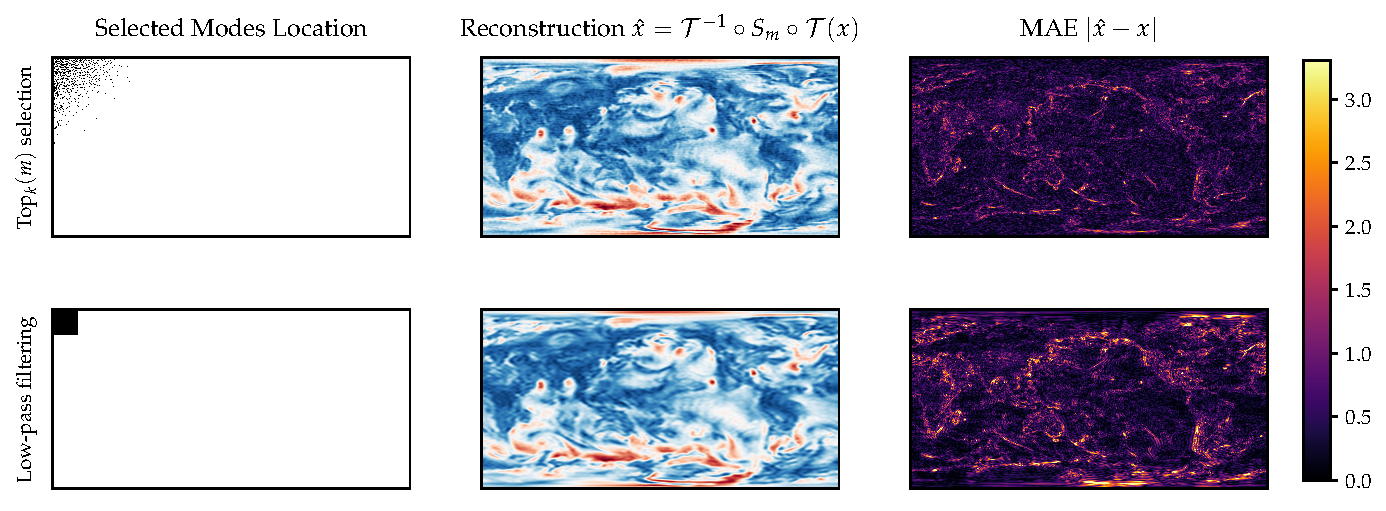
\includegraphics[width=\linewidth]{figures/era5.pdf}
    \vspace{-5.5mm}
    \caption{Reconstructions after low-pass filtering (first $m$ modes) \textbf{[Bottom]} or top-$m$ selection \textbf{[Top]} of ERA5 \citep{hersbach2020era5} climate data. The non-monotonic structure of the spectrum implies more accurate reconstructions can be obtained with top-$m$ selection.}
    \vspace{-5mm}
    \label{fig:era5}
\end{figure}

\paragraph{Mode selection criteria in general tasks} When $Y\neq X$ and the task is a general prediction task, the simple $\topk{m}$ analysis is not optimal. Nonetheless, given a dataset of input-output signals it is still possible to perform an \textit{a priori} analysis on $R_o$ to inform the choice of the best modes to keep. 

Often, we empirically observe the irreducible error $R_o$ for reduced-order \ourmethod{} to be smaller than for non-reduced-order FDMs i.e $R_o <\sum_{k=m}^{K-1}\|Y_k - \cT_k(\hat y)\|$ with layers of type \eqref{eq:1}\footnote{See \cref{fig:navier} and Appendix B for experimental evidence in support of this phenomenon.}.

We also note that the reachable component $J_\theta$ of the objective cannot always be minimized to zero regardless of the approximation power of $\gamma_{\theta}$. For each $k<m$, $S_m$ discards $N-m$ frequency components of the input signal which, if different than zero, likely contain the necessary information to approximate $\psi_k(X)$ exactly. Specifically, the irreducible lower bound on $J_\theta$ should depend on ``how much'' the output's $m$ frequency components depend on the discarded $N - m$ input's elements. 

A rough quantification of such bound can be obtained by inspecting the mismatch between the gradients of $\psi_k - \gamma_{\theta,k}\circ S_m$ with respect to $X$. In particular, it holds 
%
\[
    \sum_{j=0}^{N-1}\left|\frac{\partial\psi_k(X)}{\partial X_j} - \frac{\partial\gamma_{\theta,k}(S_m X)}{\partial X_j}\right| = \sum_{j=0}^{m-1}\left|\frac{\partial\psi_k(X)}{\partial X_j} - \frac{\partial\gamma_{\theta,k}(S_mX)}{\partial X_j}\right| + \sum_{j=m}^{N-1}\left|\frac{\partial\psi_k(X)}{\partial X_j}\right|,
\]
%
Unless $\partial_{X_j}\psi_k(X) = 0$ holds for all $j = m, \dots, N-1$ and $k = 0, 1, \dots, N-1$ i.e. no dependency of the ground truth map in $k$-space on the truncated elements, there will be an irreducible overall gradient mismatch and thus a nonzero $J_\theta$.


\subsection{Weight Initialization for Reduced-Order FDMs}\label{subsec:init}
%

FDMs \citep{li2020fourier,tran2021factorized,wen2022u} opt for a standard Xavier-like \citep{glorot2010understanding} initialization distribution that takes into account the input channels $c$ to a layer i.e. $\cN(0, \frac{1}{c})$. However, well-known variance preserving properties of Xavier schemes do not hold for FDM layers truncating $N - m$ elements of the $k$-space. Notably, Xavier schemes do not scale the variance of the weight initialization distribution based on the number of elements $m$ kept after truncation of the spectrum performed by $f_\theta$, leading to the \textit{collapse} of the outputs to zero. 


To avoid this issue in \ourmethod{} and other FDMs, we develop a simple \textit{variance-preserving} (vp) that introduces a variance scaling factor based on $m$ and the class of transform. 


{
\begin{restatable}[Variance Preserving ({\tt vp}) Initialization]{thm}{vpinit}\label{thm:vp}
%
Let $\hat x = W^* S_m^\top A S_m W x$ be a $k$-space reduced-order layer and $W$ is a normalized DCT-II transform. If $x\in\R^N$ is a random vector with 
%
\[
    \bE[x] = \0, \quad~ \mathbb{V}[x] = \sigma^2 \Id.
\]
%
Then,
%
\[
   A_{ij} \sim \mathcal{N}\left(0, \frac{{N}}{m^2}\right) \Rightarrow \mathbb{V}[\hat x] = \mathbb{V}[x].
\]
%
\end{restatable}
}


We report the proof in Appendix A, including some considerations for specific forms of $f_\theta$.
%
{
\begin{restatable}[{\tt vp} initialization for DFTs]{corollary}{vpdft}\label{cor:vp_dft}
    Under the assumptions of Theorem \ref{thm:vp}, if $W$ is a normalized DFT matrix we have $\Re(A_{ij}),\Im(A_{ij}) \sim \mathcal{N}(0, \frac{N}{2m^2}) \Rightarrow \mathbb{V}[\hat x] = \mathbb{V}[x]$.
\end{restatable}
}
%

%
The collapse phenomenon is empirically shown in  \cref{fig:vpfig} for $m=24$, comparing a single layer of FNO and FFNO (with Xavier initialization) with FNO equipped with the proposed {\tt vp} scheme. Under the assumptions of Corollary \ref{cor:vp_dft}, we sample $A$ and compute empirical variances of $\hat x = W^*S_m^\top A(\theta)S_mWx$ for several finite batches of input signals $x$. We repeat the experiment for signals of different lengths $N$. The {\tt vp} scheme preserves unitary variances whereas the other layers concentrate output variances towards zero at a rate that grows with $N - m$.
%
\begin{figure}[H]
    \vspace{-1mm}
    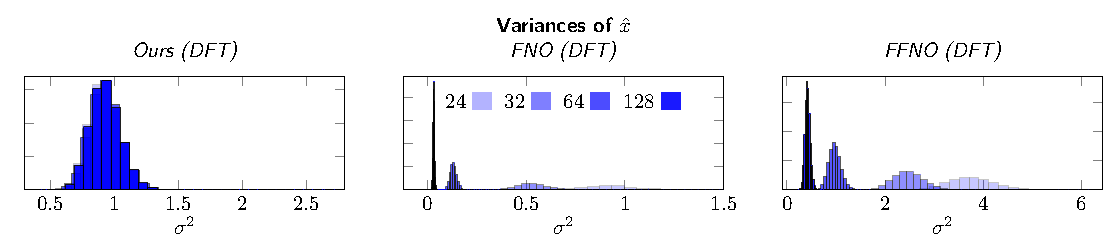
\includegraphics[width=\linewidth]{drawings/vp_hist.pdf}
    \vspace{-8mm}
    \caption{\small Output variance histogram in layer outputs $\hat x = W^*_mS_m^\top A(\theta) S_m W_N$, for a finite sample of inputs $x$ and a single sample of $\theta$. Color indicates signal resolution.}
    \label{fig:vpfig}
\end{figure}
% 
\vspace{-6mm}
When the learned frequency-domain transformation $f_\theta$ is obtained, instead of the single low-rank linear layer $f_\theta = A(\theta) S_m X$, as the composition of several layers, preserving variances can be achieved by applying the {\tt vp} scheme only to the first layer. For some variants of FDMs e.g. FNO that truncate the spectrum at each layer, {\tt vp} initialization should instead be applied to all.

